\documentclass[twoside]{article}
\input{ISC18-english.sty}
%%%%%%%%%%%%%%%%%%%%%%%%%%%%  Make sure to compile twice for proper cross-references. %%%%%%%%%%%%%%%%%%%%%%%
%%%%%%% For proper display of references, compile the document twice. %%%%%%%%%%%%%%%%%%%%% 
%%%%%%%%%%%%%%% If using TeX Live, compile using pdflatex command %%%%%%%%%%%%%%%%%%%%%%%
\begin{document}
\thispagestyle{empty}
%%%%%%%%%%%%%%%%% Article title header  %%%%%%%%%%%%%%%%%%%%
\fancyhead[LE]{Joint Parameter Estimation in the Pareto Model}
%%%%%%%%%%%%%%%%% Article authors header   %%%%%%%%%%%%%%%%%%%%
\fancyhead[RO]{Asgharzadeh, Saadati Nik}
\begin{center}
{
\includegraphics [height=25mm, width=150.3mm] {Images/isc18E}} \\
\vspace*{-1.8cm}
%\begin{center}
%\color{blue} 
%{\hspace{0.1cm}\rule{\textwidth}{1mm}}\\
%\end{center}
\vspace*{4cm}
%%%%%%%%%%%%%%%%% Article title  %%%%%%%%%%%%%%%%%%%%
{\Large \bf Joint Parameter Estimation in the Pareto Model under Type-II Censoring: A Bayesian Approach}\\
%%%%%%%%%%%%%%%%% Article authors and affiliations %%%%%%%%%%%%%%%%%%%%
{\bf
Akbar Asgharzadeh\footnote[1]{{\bf Corresponding Author:} {\tt a.asgharzadeh@umz.ac.ir }}, Ali Saadati Nik$^2$  \\
$^{1,2}$Department of Statistics, Faculty of Mathematical Sciences, University of Mazandaran, Babolsar, Iran }
\end{center}
\rule{\textwidth}{0.2mm}\\
%%%%%%%%%%%%%%%%% Article abstract  %%%%%%%%%%%%%%%%%%%%
\noindent{\bf Abstract:}\\
This paper presents a Bayesian approach for joint estimation of the two-parameter Pareto model under type-II censoring. Based on censored lifetime data, the posterior distributions of the model parameters are derived by combining the likelihood function with suitable prior distributions. A two-step procedure is developed to obtain closed-form Bayesian credible regions for the parameters.
 
\noindent{\bf Keywords:} 
Pareto distribution, Bayesian credible regions, type-II censored data. \\
\noindent{\bf Mathematics Subject Classification (2010):} $\rm 99X99$, $\rm 99X99$, $\rm 99X99$. \\
\hspace{1cm}\rule{\textwidth}{0.2mm}\\
%%%%%%%%%%%%%%
\section{Introduction}
Let us consider a two-parameter Pareto distribution with the shape parameter $\alpha$ and scale parameter $\sigma$, denoted by $\mathcal{P}(\alpha,\sigma)$, with the cumulative distribution function (cdf) and the probability density function (pdf)
%
\begin{align}
	&\mathcal{F}(x;\alpha,\sigma)=1-(\sigma x)^{-\alpha},\qquad x\ge\frac{1}{\sigma},~\alpha>0,\label{cdf-Two-Pareto}\\
	&f(x;\alpha,\sigma)=\alpha\,\sigma\, (\sigma x)^{-\alpha-1},\qquad x\ge\frac{1}{\sigma},~\alpha>0, \label{pdf-Two-Pareto}
\end{align}
%
respectively.
%

In a life-testing experiment, suppose that $n$ units are placed under observation and the test is terminated upon the occurrence of the $m$-th failure, where $m<n$. Consequently, only the first $m$ failure times are observed. This ordered sample, denoted as $X_{1:n} < X_{2:n} < \dots < X_{m:n}$, is termed a type-II censored sample. For ease of notation, we represent $X_{1:n}, \dots, X_{m:n}$ as $X_1, \dots, X_m$.

In this paper, Bayesian credible regions for the parameters of the two-parameter Pareto distribution are developed based on type-II censored data.

Confidence intervals and confidence regions provide plausible ranges for unknown parameters and are widely used across various disciplines. For example, in quality control and industrial applications, they play a crucial role in assessing product lifetimes and determining appropriate warranty periods. Numerous authors have studied the construction of confidence intervals and regions for the unknown parameters; see, for example, \cite{Asgharzadeh2017,Asgharzadeh2020}, \cite{Fernandez2012,Fernandez2013,Fernandez2023}, \cite{Lennartz2021}, \cite{Saadati-Asgharzadeh-2025,Saadati-et-al-2025}, and \cite{Wu2022}.

Suppose that $\mathbf{X}=(X_1,\dots,X_m)$ is a type-II censored sample from the $\mathcal{P}(\alpha,\sigma)$ distribution with the observed sample $\mathbf{x}=(x_1,\dots,x_m)$. The joint pdf of $\mathbf{X}=(X_1,\dots,X_m)$ is
%
\begin{align}
	f(\mathbf{x}\mid\alpha,\sigma)&\propto\prod_{i=1}^{m}f(x_i;\alpha,\sigma)\big[1-\mathcal{F}(x_m;\alpha,\sigma)\big]^{n-m}\nonumber\\
	%	&=\alpha^m\,\sigma^{-n\alpha}\,x_m^{-(n-m)\alpha}\big(\prod_{i=1}^{m}x_i\big)^{-\alpha-1}\nonumber\\
	%&=\frac{1}{\prod_{i=1}^{m}x_i}\alpha^m\,\sigma^{-n\alpha}\,\exp\left(-\alpha\Big(\sum_{i=1}^{m}\ln x_i+(n-m)\ln x_m\Big)\right)\nonumber\\
	&=\frac{1}{\prod_{i=1}^{m}x_i}\alpha^m\,\sigma^{-n\alpha}\,\exp\big(-\alpha (t_m+n\ln x_1)\big),\quad \sigma\ge \frac{1}{x_1},~\alpha>0,
	\label{likelihood-function}
\end{align}
where, $t_m$  is the observed value of $T_m=\sum_{i=1}^{m}\ln X_i+(n-m)\ln X_m-n\ln X_1$. Clearly $(T_m,X_1)$ is a minimal sufficient statistics for $(\alpha,\sigma)$. For $m\ge 2$, the maximum likelihood (ML) estimates of $\alpha$ and $\sigma$, denoted by $\widehat{\alpha}$ and $\widehat{\sigma}$, are given by
\[
\widehat{\alpha}=\frac{m}{t_m},\quad\textrm{and}\quad \widehat{\sigma}=\frac{1}{x_1}.
\]
It can be seen that the distribution of $T_m$ is gamma $\mathcal{G}(m-1, \alpha)$ distribution and $Y=\ln(\sigma X_1)\sim \textrm{Exp}(n\alpha)$ with $E(Y)=(n\alpha)^{-1}$.

Consider the joint prior distribution for parameters $(\alpha, \sigma)$ defined as:
\[
\pi(\alpha, \sigma) \propto \alpha^c\, \sigma^{\gamma\alpha - 1}\, b^{-\gamma\alpha}\,\exp(-d\alpha), \quad \alpha > 0, \quad \sigma\ge \frac{1}{b},
\]
where $\gamma$, $b$, $c$, and $d$ are positive hyperparameters. This prior is applied in Bayesian analysis of the two-parameter Pareto distribution, as noted in works by \cite{Arnold-Press} and \cite{Lwin}. The joint prior can be factored as:
\[
\pi(\alpha, \sigma) = \pi(\alpha) \, \pi(\sigma \mid \alpha),
\]
with $\alpha$ following a gamma $\mathcal{G}(c,d)$, and $\sigma \mid \alpha \sim \mathcal{P}(\gamma\alpha, b)$.

By setting $\gamma = d=0$, $c = -1$, and taking the limit as $b \to \infty$ ($b=x_1$ is sufficient), the prior simplifies to the non-informative form:
\[
\pi(\alpha, \sigma) \propto \frac{1}{\alpha \sigma}, \quad \alpha > 0, \quad \sigma > 0.
\]
So, the posterior pdf of $(\alpha,\sigma)$ given $\mathbf{X}=\mathbf{x}$ is defined by
%
\begin{align}
	\mathcal{\pi}(\alpha,\sigma\mid\mathbf{x})&=\frac{1}{c(\mathbf{x})}\,f(\mathbf{x}\mid\alpha,\sigma)\,\mathcal{\pi}(\alpha,\sigma)\nonumber\\
	&=\frac{1}{c(\mathbf{x})}\,\alpha^{m+c}\,\sigma^{-\alpha(n+ \gamma)-1}\,\exp\big(-\alpha(d+\gamma\ln b+t_m+n\ln x_1)\big),\label{posterior-pdf}
\end{align}
for $\sigma>\xi,~\alpha>0$, where, $\xi=\max\big(\frac{1}{x_1},\frac{1}{b}\big)$ and
\[
c(\mathbf{x})=\int_{0}^{\infty}\int_{\xi}^{\infty}f(\mathbf{x}\mid\alpha,\sigma)\,\mathcal{\pi}(\alpha,\sigma)\,\mathrm{d}\sigma\,\mathrm{d}\alpha=\frac{\Gamma(m+c)}{(n+\gamma)\,\big(\omega+t_m+n\ln x_1\big)^{m+c}},
\]
with, $\omega=d+\gamma\ln (b\xi)+n\ln\xi$.
%So,
%
%\begin{equation}\label{posterior-pdf}
%	\mathcal{\pi}(\alpha,\sigma\mid\mathbf{x})=\frac{(n+\gamma)\,\big(\omega+t_m+n\ln x_1\big)^{m+c}}{\Gamma(m+c)}
%	\alpha^{m+c}\,\sigma^{-\alpha(n+\gamma)-1}\,\exp\big(-\alpha(d+\gamma\ln b+t_m+n\ln x_1)\big),	
%\end{equation}
%for $\sigma>\xi,~\alpha>0$.

\begin{cor}\label{alpha-marginal-corollary}
	The conditional posterior density of $\alpha$ given the data $\mathbf{x}$ is expressed as:
	%
	\begin{align*}
		\pi(\alpha \mid \mathbf{x}) &= \int_\xi^\infty \pi(\alpha, \sigma \mid \mathbf{x}) \, \mathrm{d}\sigma\\
		&	= \frac{(\omega+t_m+n\ln x_1)^{m + c}}{\Gamma(m + c)}\, \alpha^{m + c-1}\,\exp\big(-\alpha(\omega+t_m+n\ln x_1)\big), 	
	\end{align*}
	%
	for $\alpha > 0$. Evidently, $\alpha \mid \mathbf{x}$ follows a gamma  $\mathcal{G}(m + c, \omega+ t_m+n\ln x_1)$.
\end{cor}
%%
%
\begin{cor}\label{conditional-sigma-corollary}
	%
	Using the posterior distribution, the conditional posterior density of $\sigma$ given $\alpha$ and the data $\mathbf{x}$ is derived as:	
	\[
	\pi(\sigma \mid \alpha, \mathbf{x}) = \frac{\pi(\alpha, \sigma \mid \mathbf{x})}{\pi(\alpha \mid \mathbf{x})} = \alpha (n + \gamma)\,\xi^{\alpha (n + \gamma)}\, \sigma^{-\alpha (n + \gamma) - 1}, \quad  \sigma > \xi.
	\]	
	It follows that the transformed variable $Y = \frac{\xi}{\sigma} \mid (\alpha, \mathbf{x})$ follows a Beta distribution, specifically $\text{Beta}(\alpha (n + \gamma), 1)$.
\end{cor}





\section{Credible regions} \label{closed-form-region}

This section outlines a two-step procedure to construct a $100(1 - \zeta)\%$ Bayesian credible region for the parameters $(\alpha, \sigma)$, leveraging Corollaries \ref{alpha-marginal-corollary} and \ref{conditional-sigma-corollary}. The algorithm proceeds as follows:
\begin{enumerate}
	\item[] \textbf{Step 1.}
	Determine a $100(\sqrt{1 - \zeta})\%$ credible interval \(\Lambda\) for \(\alpha\) using the marginal posterior distribution \(\pi(\alpha \mid \mathbf{x})\) from Corollary \ref{alpha-marginal-corollary}. Given that \(\alpha \mid \mathbf{x} \sim \mathcal{G}(m + c , \omega + t_m+n\ln x_1)\), the transformed variable $2(\omega + t_m+n\ln x_1)\alpha \mid \mathbf{x}$ follows a chi-square distribution with $2m + 2c$ degrees of freedom, i.e., $2(\omega + t_m+n\ln x_1)\alpha \mid \mathbf{x} \sim \chi^2(2m + 2c)$. We have
	\[
	\text{Pr}\left[\chi^2_{\zeta^-}(2m + 2c) < 2(\omega + t_m+n\ln x_1)\alpha < \chi^2_{\zeta^+}(2m + 2c) \mid \mathbf{x}\right] = \sqrt{1 - \zeta},
	\]
	which is equivalent to:
	\[
	\text{Pr}\left[\frac{\chi^2_{\zeta^-}(2m + 2c)}{2(\omega + t_m+n\ln x_1)} < \alpha < \frac{\chi^2_{\zeta^+}(2m + 2c)}{2(\omega + t_m+n\ln x_1)} \mid \mathbf{x}\right] = \sqrt{1 - \zeta},
	\]
	where, $\zeta^-=\frac{1-\sqrt{1-\zeta}}{2}$ and $\zeta^+=\frac{1+\sqrt{1-\zeta}}{2}$.
	Thus, the credible interval for $\alpha$ is:
	\[
	\Lambda = \left\{\alpha : \frac{\chi^2_{\zeta^-}(2m + 2c)}{2(\omega + t_m+n\ln x_1)} < \alpha < \frac{\chi^2_{\zeta^+}(2m + 2c)}{2(\omega + t_m+n\ln x_1)} \mid \mathbf{x}\right\}.
	\]
	%
	\item[] \textbf{Step 2.}
	For each $\alpha \in \Lambda$, construct a $100(\sqrt{1 - \zeta})\%$ credible interval $\mathcal{D}(\alpha)$ for $\sigma$ based on the conditional posterior $\pi(\sigma \mid \alpha, \mathbf{x})$ from Corollary \ref{conditional-sigma-corollary}. Since $\pi(\sigma \mid \alpha, \mathbf{x})$ is an decreasing function of $\sigma$ over the interval $(\xi, \infty)$, define the interval as:
	\[
	\mathcal{D}(\alpha) = \left\{\sigma \in (\xi, k) : \int_\xi^k \pi(\sigma \mid \alpha, \mathbf{x}) \, \mathrm{d}\sigma = \sqrt{1 - \zeta}\right\},
	\]
	yielding the solution $k = \xi/ \left(1 - \sqrt{1 - \zeta}\right)^{\frac{1}{\alpha(n + \gamma)}}$.
	
	The $100(1-\zeta)\%$ Bayesian credible region for $(\alpha, \sigma)$, denoted $\mathcal{C}^{\text{Bys}}$, is given by:
	%
	\begin{align}
		\mathcal{C}^{\text{Bys}} = \Biggl\{ (\alpha, \sigma):~& \frac{\chi^2_{\zeta^-}(2m+2c)}{2(\omega + t_m+n\ln x_1)} < \alpha < \frac{\chi^2_{\zeta^+}(2m+2c)}{2(\omega + t_m+n\ln x_1)},\nonumber \\
		& \xi< \sigma < \frac{\xi}{ \left(1 - \sqrt{1 - \zeta}\right)^{\frac{1}{\alpha(n + \gamma)}}} \Biggr\}.\label{BS-Eq-region1}	
	\end{align}
\end{enumerate}
%
The area of the region $\mathcal{C}^{\textrm{Bys}}$ is
\begin{align}
	\textrm{Area}[\mathcal{C}^{\text{Bys}}]&=\iint\limits_{\mathcal{C}^{\text{Bys}}}\,\mathrm{d}\sigma\,\mathrm{d}\alpha\nonumber\\
	&=\xi\int_{\frac{\chi^2_{\zeta^-}(2m+2c)}{2(\omega+t_m+n\ln x_1)}}^{\frac{\chi^2_{\zeta^+}(2m+2c)}{2(\omega+t_m+n\ln x_1)}}\Big(\left(1 - \sqrt{1 - \zeta}\right)^{\frac{-1}{\alpha(n + \gamma)}}-1\Big)\,\mathrm{d}\alpha.\label{BS-area}
\end{align}





\section{Illustrative example}\label{example-section}
In this section, an numerical example is provided for illustration. The example is based on a Pareto data set reported by \cite{Hong-et-al} on business failures. The underlying
random variable, $X$, denotes the length of time in years for which a business operates until failure. Only the 65 smallest
failure times were observed in a sample of 200 businesses. Business operational lifetimes are displayed in Table \ref{business-failures-data}. For this data, $x_1=1.02$ is the first failure time and $t_m=654.264$ is the observed value of $T_m$.

%
\begin{table}[ht!]
	\small
	\caption{Business operational lifetimes}\label{business-failures-data}
	%
	\setlength{\tabcolsep}{.63mm}
	\renewcommand{\arraystretch}{1.1}
\begin{center}
		\begin{tabular}{lllllllllllllllllllllllll}
		\hline
		1.02&& 1.08&& 1.09&& 1.11&& 1.12&& 1.22&& 1.42&& 1.45&& 1.57&& 1.59&& 1.62&& 1.62&& 1.74\\
		%
		1.94&& 1.94&& 1.96&& 1.99&& 2.08&& 2.32&& 2.88&& 3.01&& 3.22&& 3.65&& 3.75&& 4.11&& 4.15\\
		%
		4.26&& 4.38&& 4.71&& 4.80&& 5.47&& 5.74&& 6.38&& 6.74&& 7.42&& 7.44&& 7.60&& 7.81&& 8.46\\
		%
		8.65&& 8.92&& 10.93&& 13.02&& 15.19&& 16.16&& 16.23&& 19.59&& 19.81&& 20.16&& 20.64&& 21.32&& 23.67\\
		%
		24.04&& 25.41&& 28.77&& 30.20&& 30.66&& 31.29&& 34.37&& 45.04&& 47.62&& 48.14&& 50.74&& 51.50&& 52.68\\
		\hline
	\end{tabular}
\end{center}	
\end{table}

To derive the Bayesian credible regions, we consider the non-informative prior.  Assuming that the confidence level $1-\zeta$ is $0.90$ and $0.95$, the corresponding 95\% and 90\% Bayesian credible regions $\mathcal{C}^{\textrm{Bys}}$ are obtained as follows: 
\begin{align*}
	&\mathcal{C}^{\textrm{Bys}}_{0.95}=\Bigl\{(\alpha,\sigma):~ 0.0725<\alpha<0.1271,~\,0.9803<\sigma<\frac{0.9803}{(0.0253)^{\frac{1}{200\alpha}} }\Bigr\},\\
	&\mathcal{C}^{\textrm{Bys}}_{0.90}=\Bigl\{(\alpha,\sigma):~ 0.0754<\alpha<0.1230,~\,0.9803<\sigma<\frac{0.9803}{(0.0513)^{\frac{1}{200\alpha}} }\Bigr\}.	
\end{align*}
%
The areas of $\mathcal{C}^{\textrm{Bys}}_{0.95}$ and $\mathcal{C}^{\textrm{Bys}}_{0.90}$ are $0.0111$ and $0.0077$, respectively.
For comparison, the 95\% and 90\% Bayesian regions  $\mathcal{C}^{\textrm{Bys}}$ are illustrated in Figure \ref{compare-figure1}.

\begin{figure}[ht!]
	\centering
	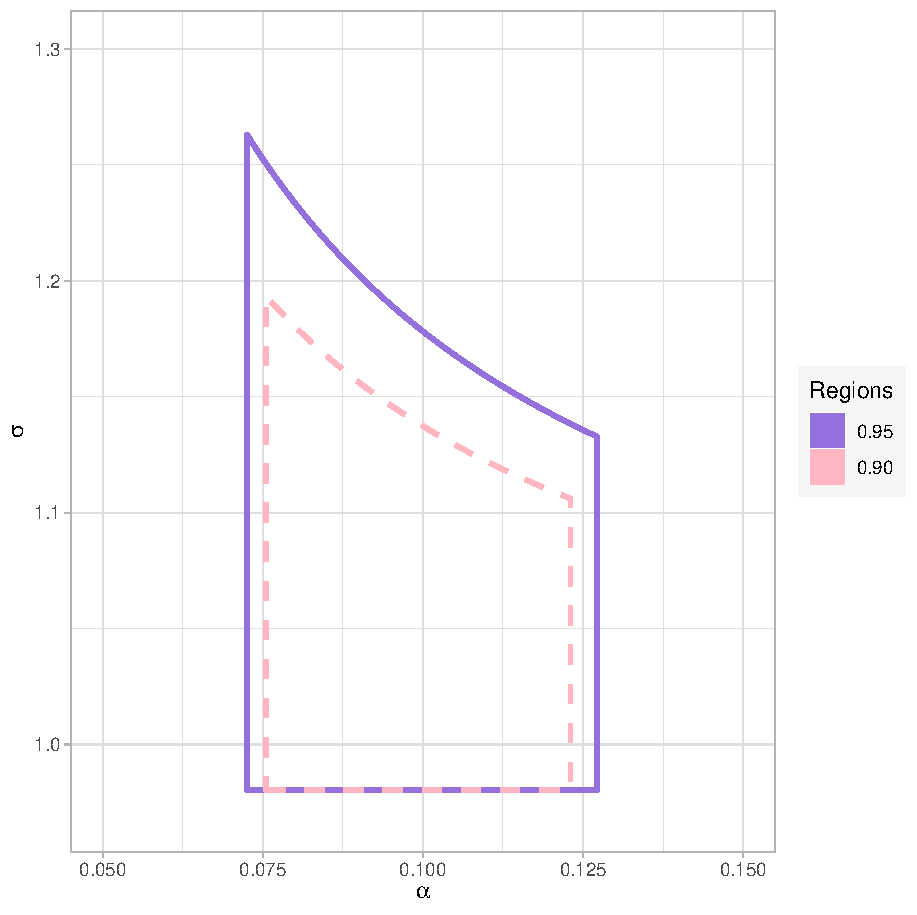
\includegraphics[scale=.4]{Images/compare-region}
	\caption{\footnotesize{Bayesian confidence regions for $(\alpha,\sigma)$.}}\label{compare-figure1}
\end{figure}



\section*{Acknowledgments}   
This research was financed by a research grant from the University of Mazandaran.



%%%%%%%%%%%%%%%%%%%%%%%% References %%%%%%%%%%%%%%%%%%%%%%%%%%%%%



\begin{thebibliography}{9}
	
	\bibitem[Arnold and Press(1989)]{Arnold-Press}
	Arnold, B.C. and Press, S.J. (1989). Bayesian estimation and prediction for Pareto data, \textit{Journal of the American Statistical Association}, 84, 1079-1084.
	
	\bibitem[Asgharzadeh et al.(2017)]{Asgharzadeh2017} Asgharzadeh, A., Fern\'andez, A.J., \& Abdi, M. (2017). Confidence sets for the two-parameter Rayleigh distribution under progressive censoring. \textit{Applied Mathematical Modeling}, 47, 656-667.
	
	\bibitem[Asgharzadeh et al.(2020)]{Asgharzadeh2020} Asgharzadeh, A., Bagheri, S.F., Ibrahim, N.A., \& Abubakar, M.R. (2020). Optimal confidence regions for the two-parameter exponential distribution based on records. \textit{Computational Statistics}, 35, 309–326.
	
	\bibitem[Fern\'{a}ndez(2012)]{Fernandez2012} Fern\'{a}ndez, A.J. (2012). Minimizing the area of a Pareto confidence region. \textit{European Journal of Operational Research}, 221, 205-212.
	
	\bibitem[Fern\'{a}ndez(2013)]{Fernandez2013} Fern\'{a}ndez, A.J. (2013). Smallest Pareto confidence regions and applications. \textit{Computational Statistics} \& \textit{Data Analysis}, 62, 11–25.	
	
	\bibitem[Fern\'{a}ndez(2023)]{Fernandez2023} Fern\'{a}ndez, A.J. (2023). Optimal Confidence Regions for Weibull Parameters and Quantiles under Progressive Censoring. \textit{Algorithms}, 16, 427. \url{https://doi.org/10.3390/a16090427}
	
	\bibitem[Hong et al.(2008)]{Hong-et-al}  Hong, C.-W., Wu, J.-W., Cheng, C.-H. (2008). Computational procedure of performance assessment of lifetime index of Pareto lifetime businesses based on
	confidence interval. \textit{Applied Soft Computing}, 8, 698–705.
	%
	
	\bibitem[Lennartz et al.(2021)]{Lennartz2021}
	Lennartz, J.M., Bedbur, S., and Kamps, U. (2021).
	Minimum area confidence regions and their coverage probabilities for type-II censored exponential data.
	\textit{Statistical Papers}, 62, 171–191.
	\url{https://doi.org/10.1007/s00362-019-01087-x}
	
	\bibitem[Lwin(1972)]{Lwin}
	Lwin, T. (1972). Estimation of the tail of the Paretian law, \textit{Skand Aktuarietidskr}, 55, 170-178.
	
	\bibitem[Saadati Nik and Asgharzadeh(2025)]{Saadati-Asgharzadeh-2025}
	Saadati Nik, A., and Asgharzadeh, A. (2025).
	Bayesian joint estimation for the two-parameter exponential distribution based on records.
	\textit{Communications in Statistics – Theory and Methods}, 1–15.
	\url{https://doi.org/10.1080/03610926.2025.2560035}
	
	
	\bibitem[Saadati Nik et al.(2025)]{Saadati-et-al-2025}
	Saadati Nik, A., Asgharzadeh, A., and Fern\'{a}ndez, A.J. (2025).
	Bayesian credible regions for two-parameter exponential distributions under Type-II censoring.
	\textit{Journal of Computational and Applied Mathematics}, 470, 116721.
	\url{https://doi.org/10.1016/j.cam.2025.116721}
	
	\bibitem[Wu(2022)]{Wu2022}
	Wu, S.F. (2022).
	Interval estimation for the two-parameter exponential distribution under progressive type-II censoring on the Bayesian approach.
	\textit{Symmetry}, 14, 808.
	\url{https://doi.org/10.3390/sym14040808}
	
\end{thebibliography}



 \end{document}

